\section{}
\[
H(s)=\frac{4}{s^2-4}=\frac{4}{(s-2)(s+2)}\,.
\]
\subsection{Bode-Diagramm}
\begin{center}
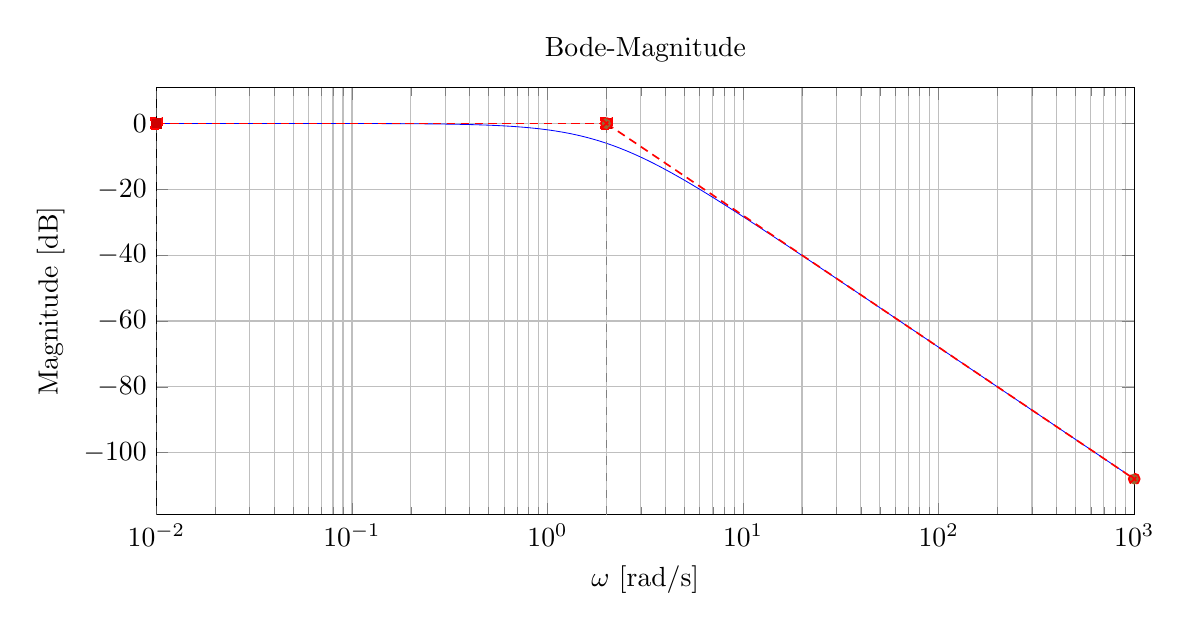
\begin{tikzpicture}
\begin{semilogxaxis}[
  width=14cm,height=7cm,
  xmin=1e-2,xmax=1e3,
  xlabel={$\omega$ [rad/s]},
  ytick distance=20,
  ylabel={Magnitude [dB]},
  grid=both,
  title={Bode-Magnitude}
]
\addplot[
  domain=1e-2:1e3,
  samples=800,
  mark=none,
  line width=0.3pt,
  blue
] {-40*ln(sqrt(1 + (x/2)^2))/ln(10)};
\addplot+[domain=1e-2:2,samples=2,dashed,dash pattern=on 3pt off 2pt,line width=0.6pt,red] {0};
\addplot+[domain=2:1e3,samples=2,dashed,dash pattern=on 3pt off 2pt,line width=0.6pt,red] {-40*ln(x/2)/ln(10)};
\draw[gray,dashed] (rel axis cs:0,0) -- (rel axis cs:0,1);
\draw[gray,dashed] (axis cs:2,\pgfkeysvalueof{/pgfplots/ymin}) -- (axis cs:2,\pgfkeysvalueof{/pgfplots/ymax});
\node[gray,anchor=south east] at (axis cs:2,\pgfkeysvalueof{/pgfplots/ymax}) {\scriptsize Pole $\omega_p=2$ (LHP \& RHP)};
\end{semilogxaxis}
\end{tikzpicture}
\vspace{6mm}
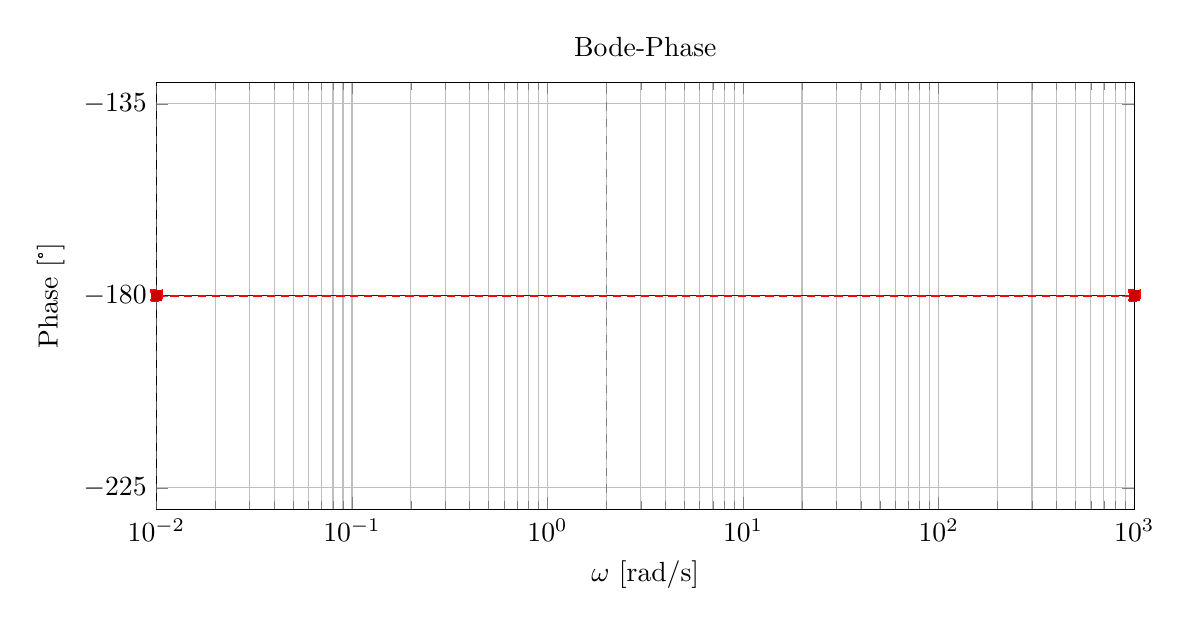
\begin{tikzpicture}
\begin{semilogxaxis}[
  width=14cm,height=7cm,
  xmin=1e-2,xmax=1e3,
  ymin=-230,ymax=-130,
  ytick distance = 45,
  xlabel={$\omega$ [rad/s]},
  ylabel={Phase [°]},
  grid=both,
  title={Bode-Phase}
]
\addplot[
  domain=1e-2:1e3,
  samples=2,
  mark=none,
  line width=0.3pt,
  blue
] {-180};
\addplot+[domain=1e-2:1e3,samples=2,dashed,dash pattern=on 3pt off 2pt,line width=0.6pt,red] {-180};
\draw[gray,dashed] (rel axis cs:0,0) -- (rel axis cs:0,1);
\draw[gray,dashed] (axis cs:2,\pgfkeysvalueof{/pgfplots/ymin}) -- (axis cs:2,\pgfkeysvalueof{/pgfplots/ymax});
\node[gray,anchor=south east] at (axis cs:2,\pgfkeysvalueof{/pgfplots/ymax}) {\scriptsize Pole $\omega_p=2$ (LHP \& RHP)};
\end{semilogxaxis}
\end{tikzpicture}
\end{center}
\newpage
\subsection{Erklärung (ausführlich)}
\begin{description}[leftmargin=1.2em,labelsep=.6em,font=\bfseries]

\item[1. Normalform herstellen.]
\[
H(s)=\frac{4}{(s-2)(s+2)}
= K_0\cdot\frac{1}{(1-sT_{p1})}\cdot\frac{1}{(1+sT_{p2})}
\]
mit
\[
K_0=-1,\quad r=0,\quad T_{p1}=\tfrac{1}{2},\quad T_{p2}=\tfrac{1}{2}.
\]

\item[2. Eckfrequenz bestimmen und sortieren.]
\[
\omega_{p1}=\tfrac{1}{T_{p1}}=\omega_{p2}=\tfrac{1}{T_{p2}}=2\,\mathrm{rad/s}
\]

\item[3. Startpunkt des Amplitudengangs festlegen.]
Setze \(\omega_{\min}=\omega_p=2\).
\[
F_{\mathrm{dB}}(\omega_{\min})=20\log_{10}\!\big(|K_0\,\underline{F}^*_{\mathrm{ges}}(0)|\,\omega_{\min}^{\,r}\big)
=20\log_{10}(1)=0\,\mathrm{dB}.
\]
Ankerpunkt: \(0\,\mathrm{dB}\) bei \(\omega=2\).

\item[4. Verlauf links vom Startpunkt zeichnen.]
Für \(\omega<2\): Anfangssteigung \(r\cdot 20=0\,\mathrm{dB/dec}\) \(\Rightarrow\) horizontale Asymptote bei \(0\,\mathrm{dB}\).

\item[5. Steigungswechsel an der Eckfrequenz eintragen.]
Ab \(\omega=2\): zwei einfache Pole (RHP \& LHP) \(\Rightarrow\) zusätzliche \(-40\,\mathrm{dB/dec}\). Netto:
\[
\begin{cases}
0\,\mathrm{dB},& \omega<2,\\
-40\log_{10}(\omega/2),& \omega\ge 2.
\end{cases}
\]

\item[6. Eckabrundung korrekt berücksichtigen.]
Am Knick \(\omega=2\): Summe zweier \(-3\,\mathrm{dB}\)\ \(\Rightarrow\)\ \(-6\,\mathrm{dB}\) unter der Geraden:
\[
|H(j2)|_{\mathrm{dB}}\approx -6\,\mathrm{dB}.
\]
(Dies gilt hier trotz RHP/LHP-Mischung, da es um den \emph{Betrag} geht.)

\item[7. Phasenstartwert festlegen.]
Da \(K_0\,\underline{F}^*_{\mathrm{ges}}(0)<0\) und \(r=0\),
\[
\varphi(0)=-180^\circ + r\cdot90^\circ = -180^\circ.
\]

\item[8. Phasenänderung durch die Polglieder (Überlappung/Kompensation).]
Ein LHP-Pol trägt \(-90^\circ\) über seine Übergangsdekade \([0.2,20]\) bei, ein RHP-Pol gleicher Lage trägt \(+90^\circ\) über \([0.2,20]\) bei. Diese Beiträge überlappen vollständig und kompensieren sich zu \(0^\circ\); daher bleibt die Phase für alle \(\omega\) konstant bei \(-180^\circ\) (der durch \(K_0<0\) vorgegebene Offset).

\item[9. Grenzwerte und Konsistenz prüfen.]
DC: \(|H(0)|=1\Rightarrow 0\,\mathrm{dB}\), \(\varphi(0)=-180^\circ\).
HF: \(|H(j\omega)|=\frac{4}{\omega^2+4}\sim \frac{4}{\omega^2}\Rightarrow -40\log_{10}(\omega/2)\,\mathrm{dB}\), \(\varphi(\infty)=-180^\circ\).

\end{description}

\subsubsection*{Stückweise Näherungen (für die Skizze)}
\[
|H(j\omega)|_{\mathrm{dB}}\approx
\begin{cases}
0,& \omega\ll 2,\\[2pt]
-6,& \omega=2,\\[2pt]
-40\log_{10}(\omega/2),& \omega\gg 2,
\end{cases}
\]
\[
\varphi(\omega)\approx
\begin{cases}
-180^\circ,& \text{für alle }\omega.
\end{cases}
\]

\newpage